\labelsubsection{Results and Observations}{subsec:results_and_observations}
\todo[inline]{Observations + possible explanations}
\todo[inline]{How do the results relate to hypothesis?}
\todo[inline]{Error analysis}
\todo[inline]{Confusion matrices?}
\todo[inline]{Comparison between text n-grams and concept maps/co-occurrence graphs}
\todo[inline]{Look at concepts used in concept maps: frequency in whole corpus, ...}

\subquestionref{question:structure_diversity}

\begin{figure}[ht]
\centering
\begin{tabular}{lcccc}
{} &  \multicolumn{2}{c}{\#nodes/\#words} &  \multicolumn{2}{c}{\#edges/\#nodes} \\
{} & concept map &  co-occurrence &  concept map &  co-occurrence \\
\midrule
ling-spam       & 0.05 & 0.23 & 1.32 & 2.86 \\
ng20            & 0.05 & 0.18 & 1.38 & 2.71 \\
reuters-21578   & 0.09 & 0.21 & 1.46 & 2.86 \\
review\_polarity & 0.08 & 0.20 & 1.42 & 2.67 \\
rotten\_imdb     & 0.09 & 0.30 & 1.22 & 1.70 \\
tagmynews       & 0.13 & 0.37 & 1.30 & 1.81 \\
webkb           & 0.05 & 0.22 & 1.39 & 3.01 \\
\midrule
\O{}            & 0.08 & 0.24 & 1.36 & 2.52 \\
\bottomrule
\end{tabular}
\caption{Graph statistics. \textit{\#words} is the number of words in the whole text dataset. The \textit{\#edges/\#nodes} metric is for the co-occurrence graphs with a window size of 1. The \textit{\#nodes/\#words} metric is a compression factor. Note that, on average, the concept maps have a compression factor of 8\% compared to the 24\% of the co-occurrence graph. This means that co-occurrence graphs have approximately three times more content than concept maps. The \textit{\#edges/\#nodes} metric is an indicator for the connectedness of the graphs. The \textit{\#edges/\#nodes} metric captures the average degree of the nodes in the graphs. Looking at that metric, we also see that, on average, the co-occurrence graphs have roughly twice as much edges per node as concept maps.}
\end{figure}

\begin{figure}[ht]
\centering
\missingfigure[figcolor=white]{}
\caption{Percentage of graphs with more than one connected component. Per dataset for both concept maps and co-occurrence graphs}
\end{figure}

\begin{figure}[ht]
\centering
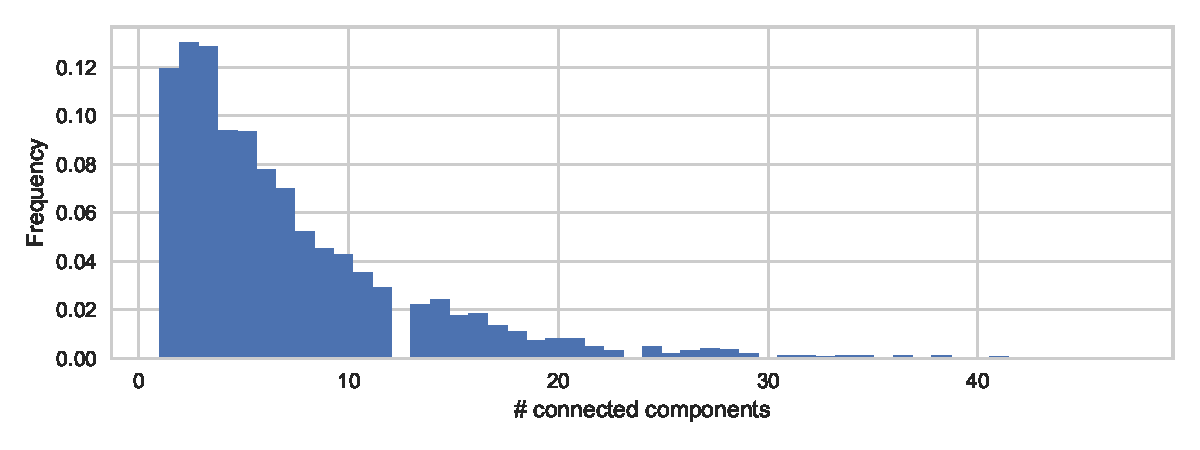
\includegraphics[width=0.8\linewidth]{assets/figures/hist-connected-components-ling-spam-CMap.pdf}
\caption{Histogram of connected components per concept map. Dataset: ling-spam.}
\end{figure}

\begin{figure}[ht]
\centering
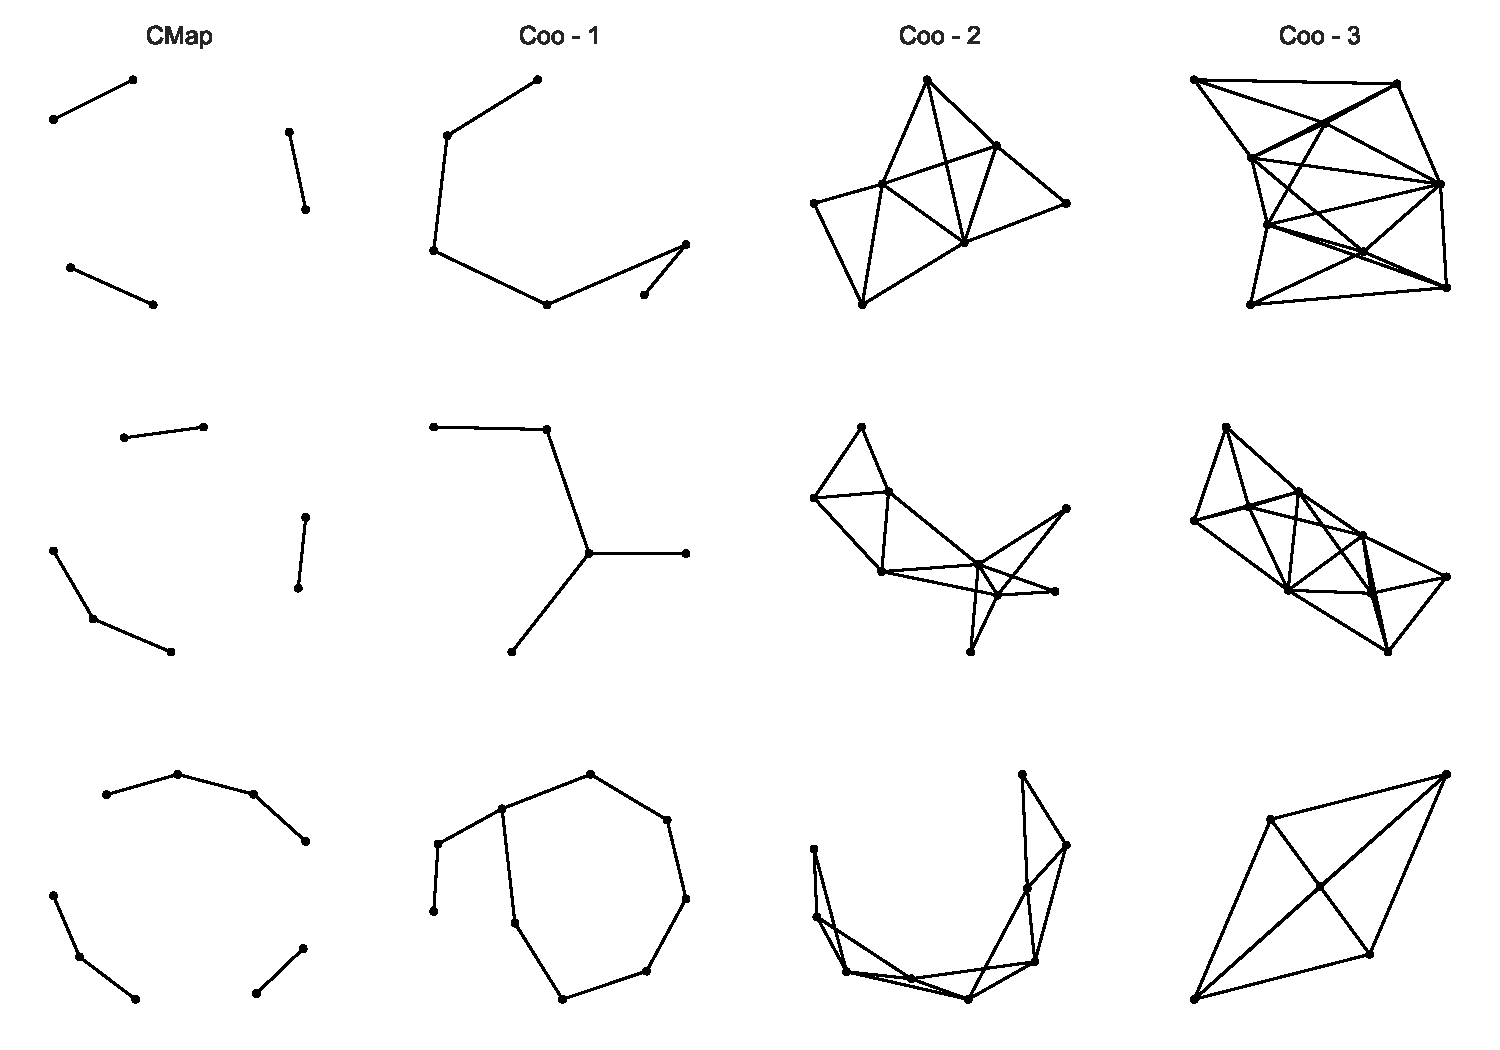
\includegraphics[width=0.6\linewidth]{assets/figures/graph-examples.pdf}
\caption{Graph examples per type. Three examples are shown per type. The concept map examples all have more than one connected component, while the co-occurrence graphs all have only one. Dataset: ling-spam}
\end{figure}

\begin{figure}[ht]
\centering
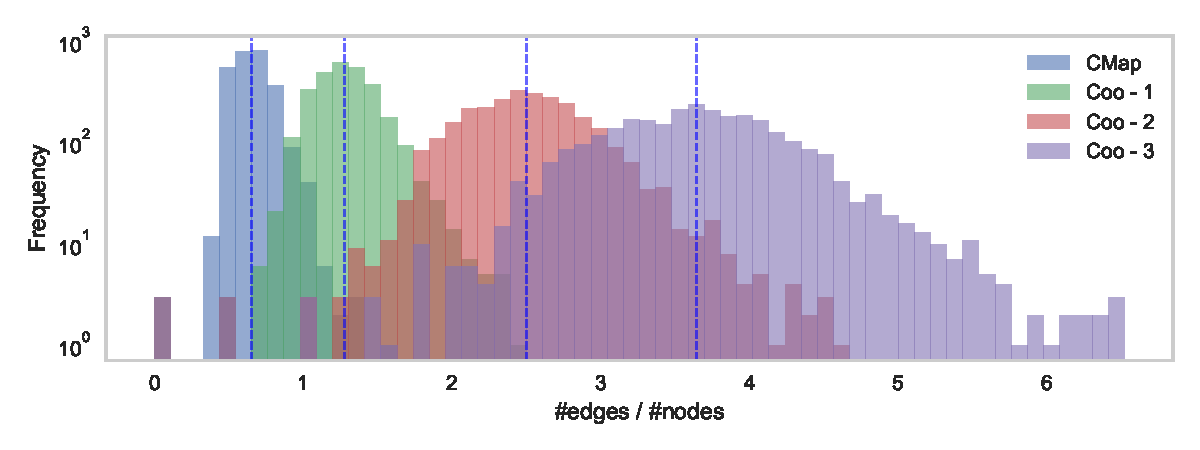
\includegraphics[width=0.7\linewidth]{assets/figures/hist-edgesnodes.pdf}
\caption{Histogram of the number of edges divided by the number of nodes. Per graph type. The lines correspond to the median value.}
\label{fig:histogram-edges-div-nodes-per-type}
\end{figure}

The co-occurrence graphs have a relatively simple structure.
Co-occurrence graphs are always connected, ie. the number of connected components is 1, or 0 in the case of an empty graph.
When the window size is 1, the graph is similar to a path, meaning that most of the nodes have a degree $< 2$. With increasing window size, the graph gets more connected.


\subquestionref{question:importance_structure}
\begin{figure}[ht]
\centering
\missingfigure[figcolor=white]{}
\caption{Comparison of linearized graph with CountVectorizer and results of WL}
\end{figure}

\begin{figure}[ht]
\centering
\missingfigure[figcolor=white]{}
\caption{Comparison of WL with and without labels}
\end{figure}

\subquestionref{question:comparison_coo}
\begin{figure}[ht]
\centering
\missingfigure[figcolor=white]{}
\caption{Comparison of co-occurrence results with concept maps}
\end{figure}

\subquestionref{question:comparison_text}
\begin{figure}[ht]
\centering
\missingfigure[figcolor=white]{}
\caption{Comparison of concept maps with text}
\end{figure}

\subquestionref{question:comparison_combined}
\begin{figure}[ht]
\centering
\missingfigure[figcolor=white]{}
\caption{Comparison of classification using both concept maps and text}
\end{figure}



\labelsubsection{Related And Intermediate Observations}{subsec:related_and_intermediate_observation}
\todo[inline]{Sparsity of feature vectors}
\todo[inline]{Complexity of approach}